\chapter{Introduction}
\lhead{Chapter 1 \emph{Introduction}}
\label{chap:1}
%\autoref{chap:1}

\section{Motivation}
\label{chap:1.1}
\bigskip
\bigskip

In 1957 the first satellite in history was launched and since then thousands of other objects were placed into orbit \cite{Belward 2015, ESA 2020}. Two decades later NASA’s scientist Donald Kessler proposed a scenario, in which he theorized that the increasing density of the objects in the Low Earth Orbit (LEO) could lead to collisions with the generated space debris increase the density even further likely to result in so-called feedback collisions. The humanity today is confronted more than ever with the realization of this theory, which has gone down as Kessler Syndrome.

There have been taken many important steps towards raising the consciousness about the growing numbers of objects in space, as well as the enactment of rules regarding the related concept of carrying capacity and potential solutions like orbit allocation. However, despite the fact that coordination committees and working groups have been established and they are involved in the development of mitigation principles and guidelines, the only existing space traffic management rules deal today only with the frequency allocation used by satellites \cite{Griffin}. %"First come, first served" procedure

Due to the concern of a congestion of near-Earth orbits and their exceeding carrying capacity \cite{Somma 2019}, new ways of dealing with this situation should be created. In this scenario of limited resources, each mission before is launched needs to be carefully considered whether its benefits outweigh another mission's advantages towards society. At worst, the needs of the society should be named and based on those the missions can be prioritized according to which mission can fulfill them.

As the first area to be experimented in the aforementioned direction, the field of Earth Observation (EO) has been identified. The reason behind the selection of EO as the first group of satellites to be tested in the application, is because the calculation of the capabilities of an EO satellite is more apparent in comparison to other scientific or technological missions. Nowadays, there is no competition between the satellite and terrestrial EO industry, since the satellites provide a cheaper solution. On the other hand, in the case of telecommunication missions, the estimation of the added value that each satellite provides to the society is more complex, due to the fact that it is not yet clear whether the space-based infrastructure would be competitive to terrestrial infrastructure.

Having said that, the motivation of this thesis is to assess the added value of a planned EO mission. For this purpose, the goal is a first demonstration of this by means of an application, which will help into supplementing the space traffic management rules regarding the physical location of satellites. The creation of a database, which hosts information about the EO satellites that are currently on orbit at the LEO region, and the connection of it to the application offers additional benefits. The user can request and find out whether there are existing orbiting and operational EO satellites or constellations that produce product with certain characteristics.

In this way, not only will users be able to discover already operational missions or satellite constellation with similar properties, %and thus conclude how many of the already existing satellites
but it also can give the incentives to business entities %private and public companies or institutes
to cooperate, offer and share the data acquired from their already orbiting satellites with other organizations that seek or are interested of those. This can be a scenario beneficial for both sides, while at the same time it helps towards conserving the common space resources of LEO, as it ultimately leads to less satellites being used for the same task.

The concept of prioritization of the missions based on the additional services that they offer before being launched seems very promising. So, one objective of this thesis is to create awareness among the space industry and the society. Another one is the creation of an application, which it can contribute to the formation of legislation based on the added value of the satellites. Hence, consensus in the corresponding space traffic management committees can be reached and the mitigation of the the number of satellites that are launched can be actualized.

\bigskip
\bigskip

\newpage
\section{Scope and key assumptions}
\label{chap:scope}
\bigskip

%\textit{Edit it...}

The first part of this master thesis pertains to the theoretical framework of the discussed issue; the carrying capacity of near-Earth orbits. The points being addressed are: the growing numbers of objects in space and the reasons behind it, the mitigation guidelines, which in part address the problem of "overpopulation". The state of LEO and its critical regions, as well as the main types of EO are also analyzed.

The second part is dedicated to the development of an application, which can give the incentives to create space traffic management rules based on the orbit and capacity allocation, as well as the added value that each new satellite may have. More specifically, the concept of added value is based on the idea that each new satellite is prioritized to be launched when it provides some additional services or data to the society, which are not offered from another existing and functional satellite/ constellation.
%It is not monetary.

As it was mentioned previously, an attempt to approach the development of such application is to focus on Earth Observation (EO) satellites at LEO. All things considered, this application has three main capabilities.
%One should also calculate the bandwidths, apart from the coverage, in the case of the Communication Satellites.

\begin{itemize}
\item The first capability is that the user can define a satellite mission or constellation, which means that the number of satellites, the altitude, the orbital plane, resolution etc. is known. Then, the software can answer what is the revisit time of that defined mission, specified in terms of the latitude: either at the equator, which is the default approach considered here, or a latitude of interest to the user.
\item The second capability is the following: The characteristics of an EO product or/and key attributes that an EO satellite has, are defined. As an example, it can be products from passive imagery sensors, which have a certain revisit time and resolution. As a result, the software can provide to the user the orbital characteristics of the satellite or constellation that can supply the desired data.
\end{itemize}

An extension of this application and its capabilities is the creation of a database of Earth Observation satellites.

\begin{itemize}
\item In both mentioned capabilities of the application, the user can find out, if there are currently satellites which offer the desired properties that they had asked for and if such satellites or constellations exist, to name them.
\end{itemize}

The database contributes greatly to the creation of a well-rounded application, which can help into mitigating the problem of the growing numbers of objects in space. Since the user can find out about whether existing satellites do a certain/asked project or offer a specific service, thus he/she can decide whether a new satellite is needed to be launched based on whether the desired service is offered or not by someone else. In this way, it can also incentivize and encourage the future companies and institutes to cooperate with each other, instead of constructing/ designing/ launching all similar satellites with comparable properties or end products in what can be considered a worst-case scenario from an environmental point of view.

In a more detailed way, such a cooperation between different entities would mean that not only the data taken by the satellites could be shared between the collaborators, but also the companies could develop the interest in placing their platform/ sensors to an existing constellation operated by another company. As a result, not only data/ images are shared, but also the orbit itself and its characteristics such as its altitude, which is usually translated in terms of resolution in the field of EO. All in all, future regulation could foresee rules reflecting on the added value any new satellite mission provides.
%For example, if you define a satellite and this exists in the database, then the value for competition is high, but there is no value for the environment.


%A space traffic management application towards the estimation of added value.

%Lastly, the part of the Evaluation follows, as well as parts of Summary and Conclusions and that of Future work.

\bigskip
Since the growing numbers of objects in space and the exceeding carrying capacity in the near-Earth orbits were the motives of this thesis, a research on the current launching trend should be carried out.


\bigskip
\section{Current launching trend}
\bigskip

\subsection{Active commercial space industry}
\bigskip
%Source: Space Environment Statistics \& the latest ESA's Environment Report with graphs and numbers (https://sdup.esoc.esa.int/discosweb/statistics/)

%LEO and compare with GEO
The world goes in the direction of launching mainly small satellites especially in LEO and more specifically in large constellations. As can be seen in Figure \ref{launch_traffic_LEO}, in a period of 10 years, namely since 2010, a fourfold increase occurred in the number of objects that were launched into LEO. On the other hand, the number of the launched objects in GEO has an upward trend without showing any further sharp peaks (Figure \ref{launch_traffic_GEO}). It is also worth mentioning that in both cases the majority of the objects placed into orbit have a commercial funding source.

\begin{figure}
\centering
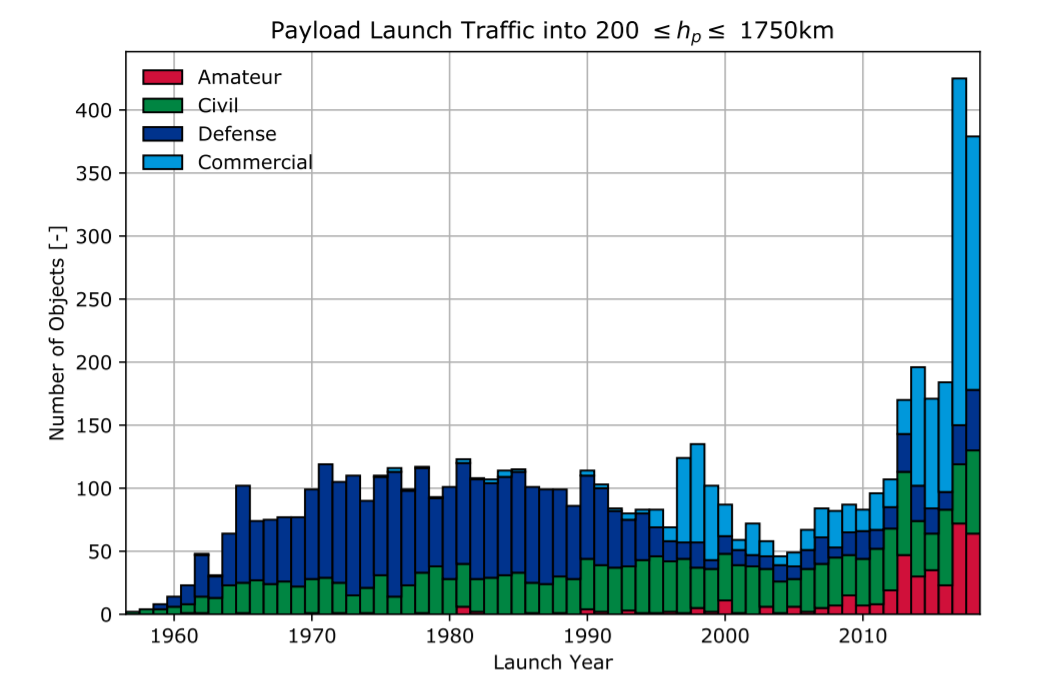
\includegraphics[width=0.9\textwidth]{Images/launch_traffic_LEO.png}\caption{Payload launch traffic into LEO (1957-2019). \textit{Source: \cite{ESA 2020}}}
\label{launch_traffic_LEO} 
\end{figure}

\begin{figure}
\centering
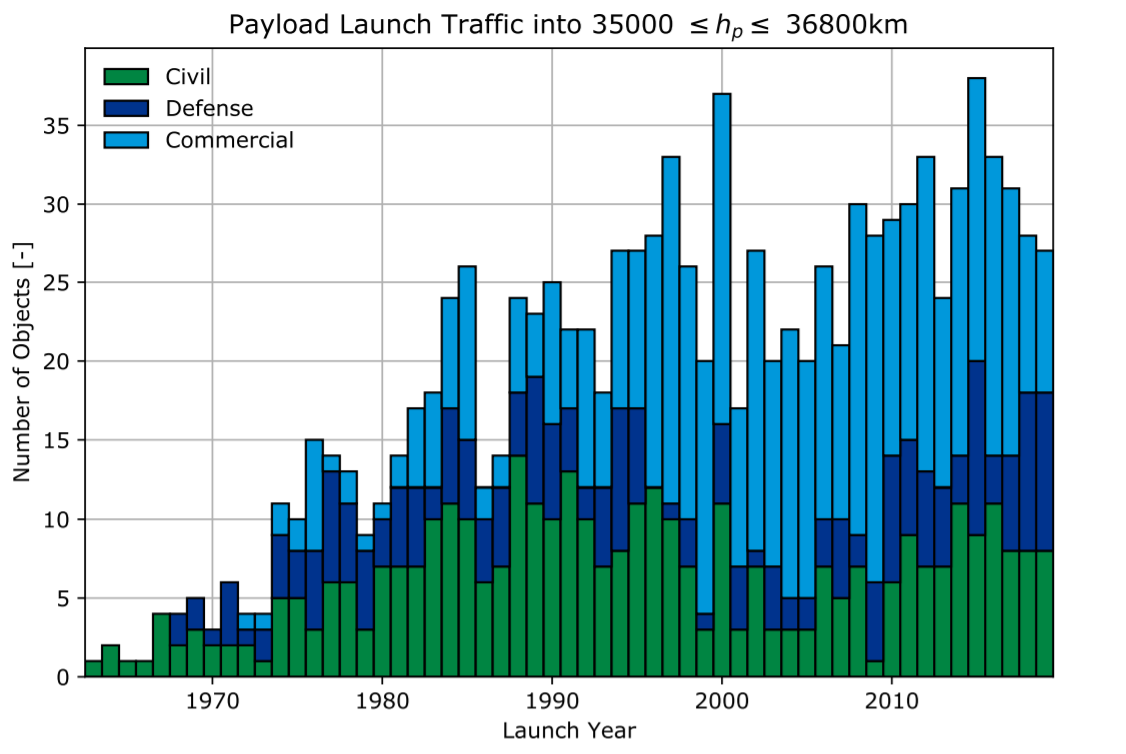
\includegraphics[width=0.9\textwidth]{Images/launch_traffic_GEO.png}\caption{Payload launch traffic into GEO (1957-2019). \textit{Source: \cite{ESA 2020}}}
\label{launch_traffic_GEO} 
\end{figure}

%Why commercial space industry is active
The reasons why the commercial space industry is more active in the last decade are various. Firstly, there is a growing demand for information services, which increases competition and reduces the costs in the market. Also, there is greater availability of capital compared to previous eras of commercial satellite growth and at the same time increasing affordability of access to space launch \cite{Hallex}. Apropos this affordable launch offers, in 2019 \textit{SpaceX} announced its rideshare program offering launch capacity for smallsats charging four to eight times cheaper than most options currently available. Since the launch is one of the most expensive aspects of a space mission, such an offer makes a big difference and creates more affordable circumstances for placing into orbit small satellites \cite{Erwin}.

\bigskip
\subsection{Proliferated constellations}
\bigskip

Another important fact is that approximately from the beginning of the millennium and for the first time in history, there is a percentage of launched objects, which are part of constellations. Moreover, since 2017 the number of objects taking part in constellations is increasing as it can be seen in Figure \ref{constellation_count_LEO}. Nevertheless, the mass of these objects has a steady course throughout this aforementioned period (Figure \ref{constellation_mass_LEO}). 

\begin{figure}
\centering
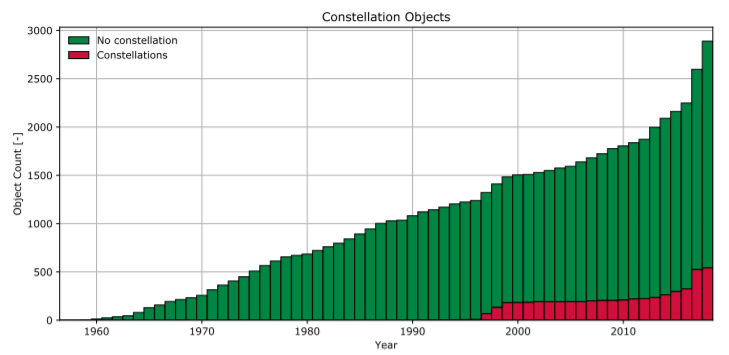
\includegraphics[width=0.9\textwidth]{Images/constellation_count_LEO.png}\caption{Evolution of number of objects as constellations at LEO. \textit{Source: \cite{ESA 2020}}}
\label{constellation_count_LEO} 
\end{figure}

\begin{figure}
\centering
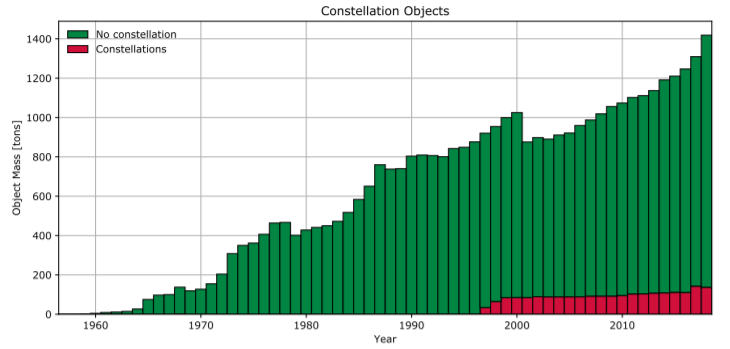
\includegraphics[width=0.9\textwidth]{Images/constellation_mass_LEO.png}\caption{Evolution of mass as constellations at LEO. \textit{Source: \cite{ESA 2020}}}
\label{constellation_mass_LEO} 
\end{figure}

The emergence of the large constellations and the further expansion of this mission design has both positive and negative effects. An important point in favor of the proliferated constellations is that they seem propitiatory for the future. This is because it provides more resilience since the loss of a satellite will not hamstring the whole constellation. Thus, the mission can continue due to the fact that there is redundancy. The proliferated constellations have in fact some drawbacks as well. Given that the large fleets are mass-produced, the performance of each and every satellite may have reduced reliability. Thus, there is a possibility of malfunction before it is retrieved. % brought back
Another drawback is that the larger a constellation is the more traffic generates. The carrying capacity is reduced, and as a result other operators may not put their satellites into similar orbit slots when there is already a large constellation in place. 

\bigskip
\subsubsection{Focused on the field of global internet}
\bigskip
%Proliferated constellations ---In persistent global internet --- Advantages n Disadvantages
The proliferated constellations are in most cases aiming at providing persistent global internet. Their focus is to provide low latency communication, which is competitive with the terrestrial broadband one for those areas where such a coverage exists. For areas with no coverage at all, it would provide basic connectivity. Despite the numerous new satellites being placed into orbit, there are some advantages of the large constellations focused on communication. As the developing world lacks access to terrestrial broadband infrastructure and almost half of the global population does not have access to the Internet, such mega-constellations appear to be helpful towards solving this problem. Another positive effect is that the laying of the costly fiber-optic cable in the developing world will be skipped. Last but not least, the high-latitude populations, such as Alaska, parts of Canada, Scandinavia, Russia, will also have the possibility of connectivity and communication with the rest of the world \cite{Hallex}.
%"Their aim is also to provide high bandwidth". + Launch of mega-constellations for satellite broadband % =ευρυζωνικότητα > Internet high-speed access.

\bigskip
\subsubsection{Focused on the field of EO}
\bigskip
%Proliferated constellations ---In EO --- Advantages n Disadvantages
Similarly to the field of communications, large constellations focused on Earth Observation have been realized. Since 2014, as can be seen in Figure \ref{launch_traffic_type_LEO}, the number of the launched payload dedicated to imaging and technology has increased rapidly. Correspondingly to the field of communication, there are several advantages of the constellations focused on EO. Many EO satellites can result in a shorter revisit time over points on Earth. This enables shorter intervals between image captures and thus the changes that appear on the ground can be easier characterized if they were driven by human activity or unanticipated events. Furthermore, the likelihood of getting a cloud-free image, or an image with fewer shadows is crucial for further analysis. They can also provide more rapid response to global events and enable imaging at times of the day previously unseen by satellites. As a result, the countries can meet carbon neutrality targets, track and quantify methane emissions and the climate change objectives are pursued \cite{LE_Esteve}. % Monitor deforestation \& human activity in general
%"This has increased the access to Earth Observation capabilities useful for national security applications."
% More notes about Planet in docx. Source: "https://www.planet.com/pulse/12x-rapid-revisit-announcement/" -Maybe not necessary to mention it.
% The ability to image all of Earth's landmass every day was reached by Planet in February 2017. 149 "Dove" satellites are (is still the same number?) orbiting Earth. [Is it an advertising?!]
%The last launching of those satellites, which were 88, is also known as "Flock 3p". Source: https://www.planet.com/pulse/planet-launches-satellite-constellation-to-image-the-whole-planet-daily/

\begin{figure}
\centering
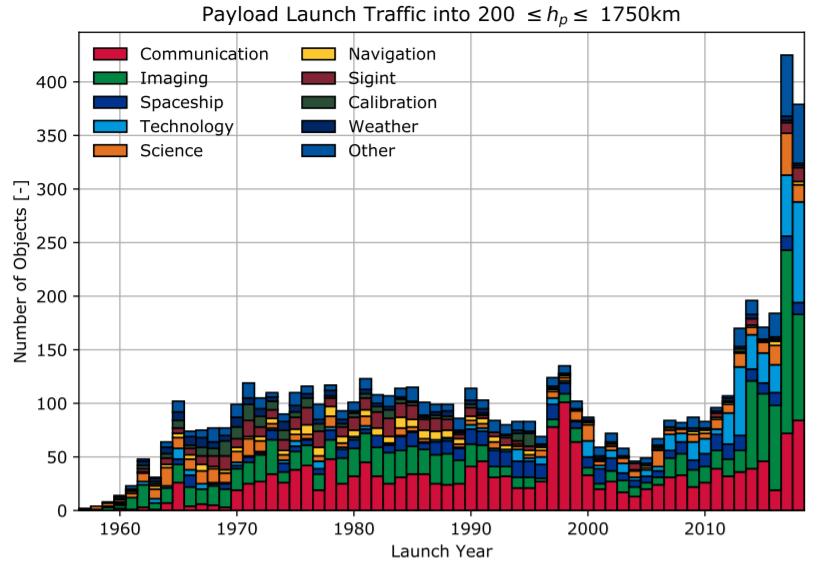
\includegraphics[width=0.9\textwidth]{Images/launch_traffic_type_LEO.png}\caption{Evolution of the launch traffic at LEO per mission type. \textit{Source: \cite{ESA 2020}}}
\label{launch_traffic_type_LEO} 
\end{figure} 

\bigskip
\subsubsection{The challenge of data handling}
\bigskip
% Many satellites == Hundreds of data / petabytes.
Besides the advantages that the services of the mega-constellations bring, there are challenges that need to be faced with regard to data handling and management. With so many satellites orbiting Earth, the existing database of EO services collectively is expected to exceed hundreds of petabytes globally. As the company \textit{Planet} forecasts, upon completion of the next \textit{Dove} constellation, there will be received up to 40 terabytes of data every day. In the same manner, the \textit{Sentinel} constellation is estimated to produce more than 20 terabytes of data per day \cite{LE_Esteve}.

\bigskip
\subsubsection{Examples of large constellations}
\bigskip
Some examples of the larger communication and EO constellations that are operated today or planned to be launched are the following. In the field of communication, the biggest constellations are operated by \textit{SpaceX} (\textit{Starlink}), \textit{Amazon} (\textit{Project Kuiper}), \textit{OneWeb}, and \textit{Telesat}. More information can be found in the Table \ref{table:internet}. Regarding the proliferated constellations of EO, the most renowned are operated by \textit{Planet, Spire Global}, and others, which can be found along with additional information in the Table \ref{table:EO}.

%By the end of 2017, Planet operated a constellation of 140 Dove imagery CubeSats, 5 RapidEye medium-resolution --> there are not operational since ~ 2015, and 13 higher resolution SkySat satellites that can image Earth’s entire landmass daily.

%In July 2018, Spire operated 61 of its Lemur satellites (out of a planned 125) that track the Automatic Identification System (AIS) beacons of ships that collect weather data by monitoring the radio occupation of GPS signals." (Table of EO constellations - in docx) --> I don't know the swath width..and what is the resolution of such a mission?
%I saw here: https://directory.eoportal.org/web/eoportal/satellite-missions/l/lemur --> "Along-track resolution = 200km" (what is it?) \cite{Hallex}

\bigskip
\begin{center}
\captionof{table}{List of the most prominent proliferated constellations in the field of internet provision. \textit{Source: \cite{Hallex, Amazon, Oneweb_bankruptcy, Kramer 2002, Hongyun, Viasat, Kepler}}}
\vspace{3mm}
\begin{adjustbox}{width=1\textwidth}
\begin{tabular}{||c| c |c |c |c |c||}
\hline
\textbf{Constellation} & \textbf{Manufacturer} & \textbf{Proposed Satellites} & \textbf{Satellite Design Life (Years)} & \textbf{Altitude (km)} & \textbf{Sat. mass (kg)}\\
\hline \hline 
Starlink $^*$ & SpaceX & 12,000 & 5-7 & 550 & 250 \\
Project Kuiper & Amazon & 3,236 %\cite{Amazon}
& n/a & 590-610 & n/a\\
OneWeb $^*$ & OneWeb & 650 %\cite{Oneweb_bankruptcy}
& 5 %\cite{Kramer 2002}
& 1,200 & 147\\
Telesat & Airbus, SSTL, SS/ Loral & 292-512 & 10 & 1,000 \& 1,250 & 150\\
Hongyun & CASIC & >150 %\cite{Hongyun}
& 1 & 1,100 & 247\\
GEN-1 $^*$ & Kepler Communications & 140 & 3-5 & 520-600 & 12-15 \\ %3U to 6U cubesats (1U is approximately 1.33kg + SSO (Sun-Synchronous Orbit). In reality the GEN-1 will be consisted of up to 15 satellites. There will be also the GEN-2 with up to 50 satellites. In total the whole Kepler constellation will be consisted of up to 140 satellites.
LeoSat & LeoSat & 78-108 & 10 & 1,400 & 1000\\
Boeing & Boeing Manufacturer & 60 %\cite{Viasat} 
& 10-15 & 1,200 & >100\\

% The company SES and the constellation O3b is operating in Geostationary and medium orbits, but there are discussions of placing satellites in LEO as well.
\hline
\end{tabular}
\label{table:internet}
\end{adjustbox}
\end{center}
\footnotesize{$^*$ {\scriptsize Already partially available as of June 2020}}
\bigskip

\normalsize

\bigskip
\begin{center}
\captionof{table}{List of the most prominent commercial proliferated constellations in the field of EO. \textit{Source: \cite{Hallex, Satellogic, Newspace, Kramer 2002}}}
\vspace{3mm}
\begin{adjustbox}{width=0.9\textwidth}
\begin{tabular}{||c| c |c |c |c||}
\hline
\textbf{Constellation} & \textbf{Manufacturer} & \textbf{Proposed Satellites} & \textbf{In orbit} (as of November 2020) & \textbf{Resolution (m)}\\
\hline \hline
Flock/ Dove & Planet & 150 & 158 & 3-5\\%Imaging the entire Earth daily
Lemur/ Minas & Spire Global, Inc. & 150 & 127 & n/a\\
Whitney & Capella Space & 40 & 1 & 1-30 (SAR)\\
Skysats (Terra Bella/ Skybox) & Planet & 21 & 21 & 0.5\\
Nusat (Aleph-1) & Satellogic & 90 & 18 & 1\\ %Argentina + Imaging the entire Earth every 2h
BlackSky & Spaceflight Industries & 60 & 6 & 1\\%It has 3 year orbital lifetime
SuperView (GaoJing) & SpaceWill (SpaceView) & 16 & 5 & 0.5\\%China
Landmapper & AstroDigital & 25 & 5 & 2.5 \& 22\\
KOMPSAT & Earth-i & 4 & 4 & 0.4-1\\
GRUS & Axelspace & 50 & 4 & 2.5\\
UrtheDaily/ OptiSar & UrtheCast & 24 & 4 & 5\\
DMC3/ TripleSat & Earth-i & 3 & 3 & 1\\
Vivid-i & Earth-i & 15 & 1 & 1\\
CE-SAT & Canon & 100 & 1 & 0.9\\%Japan
APEX, SUNSTORM & Reaktor Space & 36 & 1 & 20\\%Finland
REC & SatRevolution & 1024 & 1 & 0.5\\
HOPSAT-TD & Hera Systems & 50 & 1 & 1\\
NorthStar & NorthStar & 40 & 0 & n/a\\%Canada
WorldView Legion & Maxar & 6 & 0 & 0.3\\%Maxar: SSL, Digital Globe, MDA, Radiant
HySpec & HySpecIQ & 2 & 0 & 1\\ %EO \& Hyperspectral


%% Not exaactly Earth Observation (EO):
%HawkEye 360 --> RF Spectrum Monitoring (Mapping). It probably does geolocation: locates the geographical (latitudinal and longitudinal) location of an Internet-connected device.
%SpaceBee satellites and others - Swarm Technology (company) - Proposed satellites: 600 - In orbit: 9 (as of 10th Sept) --> It is an IOT company.

%% Others - but not much info and not large constellations:
%Triton-1,2,X (Triton 1,2 were launched in 2013 and duration was for some months. Triton-X hasn't been launched.) - LuxSpace (OHB subsidiary company)
% ESAIL (microsatellite. It was launched in Sep20. It is just one satellite in the field of ship tracking and maritime situational awareness.) - LuxSpace (OHB subsidiary company) --> https://space.skyrocket.de/doc_sdat/esail.htm

%% These are not commercial:
%Pleiades $^*$ & CNES & 2 & 0.5-2\\ (VERY OLD - 2011, 2012)
%RADARSAT (RCM) & Canadian Space Agency & 3 & SAR (1x3)m\\ (VERY OLD - 2007)
%A-train & NASA & 5 & (Goal: Hurricanes, Climate Change)\\

%% Retired constellations:
%RapidEye & Planet & 5 & 5\\
%SPOT & SPOT Image & 2 (They were 7 in total) & 1.5-6 --> Its still operating, but its VERY OLD
\hline
\end{tabular}
\label{table:EO}
\end{adjustbox}
\end{center}
%\hspace{1.5cm} \footnotesize{$^*$ {\scriptsize Already partially available as of October 2020}}
\bigskip

\normalsize

In the section \ref{app}, a table containing EO satellites of the commercial and non-commercial sector can be found (Tables \ref{table:1}, \ref{table:2}, \ref{table:3}).

Lastly, it is worth mentioning that the competition and commercialization that exists in the field of telecommunications and Earth Observation leads undeniably to the prosperity of the economy and it is also essential for preventing the creation of quasi-monopolies. Considering as a hypothetical scenario the case of \textit{Starlink}, \textit{SpaceX} while having no competitors and being successful with launching all the 12,000 proposed satellites; it will likely get its orbital altitude allocated such that no one else is able to orbit there. Therefore, for preventing such cases, the goal of the proposed application of this thesis is to recognize and encourage a virtual competition between different entities. This will help towards finding the best use of the available hardware in orbit instead of launching entire constellations and exhausting the remaining spatial resources.

% There will be competition in the lab, not in space!

All in all, NewSpace provides cheaper access to space and at the same time affordable data and services. More and more small satellites are launched in LEO in constellations, which are funded by the commercial sector. Even though this trend has several benefits, space awareness should be raised in order to promote the use of proliferated constellations \cite{pLEO}. In the same manner, by diminishing the launch rate and maintaining the growth of the services that are offered from space can lead to the reduction of space traffic. % to an extent.

%NewSpace (or Space 2.0): a movement and philosophy encompassing a globally emerging private spaceflight industry. Independent from governents and major contractors. (from Wikipedia)

%Question about title: Why the thesis can reduce space traffic? Ans: It gives the incentives. By sharing resources we have a chance to reduce space traffic.
%One question: "I want a certain EO task" --> What resolution can I have without exceeding orbit capacity?"